\documentclass{article} % For LaTeX2e
\usepackage{nips14submit_e,times}
\usepackage{amsmath}
\usepackage{amsthm}
\usepackage{amssymb}
\usepackage{mathtools}
\usepackage{hyperref}
\usepackage{url}
\usepackage{algorithm}
\usepackage[noend]{algpseudocode}
%\documentstyle[nips14submit_09,times,art10]{article} % For LaTeX 2.09

\usepackage{graphicx}
\usepackage{caption}
\usepackage{subcaption}

\def\eQb#1\eQe{\begin{eqnarray*}#1\end{eqnarray*}}
\def\eQnb#1\eQne{\begin{eqnarray}#1\end{eqnarray}}
\providecommand{\e}[1]{\ensuremath{\times 10^{#1}}}
\providecommand{\pb}[0]{\pagebreak}
\DeclarePairedDelimiter\ceil{\lceil}{\rceil}
\DeclarePairedDelimiter\floor{\lfloor}{\rfloor}

\newcommand{\E}{\mathrm{E}}
\newcommand{\Var}{\mathrm{Var}}
\newcommand{\Cov}{\mathrm{Cov}}

\newcommand{\joverline}[2]{%
  \mathord{% make sure we're in math mode
    \vbox{\offinterlineskip
      \halign{##\cr
        \hrulefill$\,\scriptscriptstyle#1\,$\hrulefill\cr
        \noalign{\kern.3ex}
        $#2$\cr
      }%
    }%
  }%
}


\def\Qb#1\Qe{\begin{question}#1\end{question}}
\def\Sb#1\Se{\begin{solution}#1\end{solution}}

\newenvironment{claim}[1]{\par\noindent\underline{Claim:}\space#1}{}
\newtheoremstyle{quest}{\topsep}{\topsep}{}{}{\bfseries}{}{ }{\thmname{#1}\thmnote{ #3}.}
\theoremstyle{quest}
\newtheorem*{definition}{Definition}
\newtheorem*{theorem}{Theorem}
\newtheorem*{lemma}{Lemma}
\newtheorem*{question}{Question}
\newtheorem*{preposition}{Preposition}
\newtheorem*{exercise}{Exercise}
\newtheorem*{challengeproblem}{Challenge Problem}
\newtheorem*{solution}{Solution}
\newtheorem*{remark}{Remark}
\usepackage{verbatimbox}
\usepackage{listings}
\usepackage{mathrsfs}
\title{Functional Analysis: \\
Problem Set III}


\author{
Youngduck Choi \\
CIMS \\
New York University\\
\texttt{yc1104@nyu.edu} \\
}


% The \author macro works with any number of authors. There are two commands
% used to separate the names and addresses of multiple authors: \And and \AND.
%
% Using \And between authors leaves it to \LaTeX{} to determine where to break
% the lines. Using \AND forces a linebreak at that point. So, if \LaTeX{}
% puts 3 of 4 authors names on the first line, and the last on the second
% line, try using \AND instead of \And before the third author name.

\newcommand{\fix}{\marginpar{FIX}}
\newcommand{\new}{\marginpar{NEW}}

\nipsfinalcopy % Uncomment for camera-ready version

\begin{document}


\maketitle

\begin{abstract}
This work contains solutions to the exercises of the problem set III.
\end{abstract}

\bigskip

\begin{question}[1]
\hfill
\begin{figure}[h!]
  \centering
    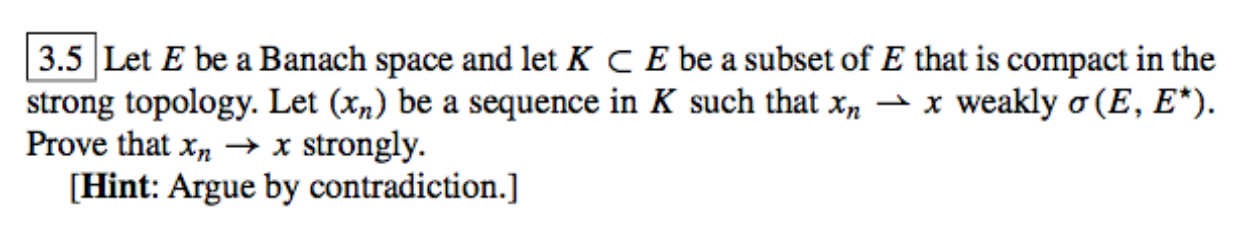
\includegraphics[width=0.7\textwidth]{funcA-h-e3-p1.png}
\end{figure}
\end{question}
\begin{solution} \hfill \\
Suppose $x_n \not\to x$ strongly. Then, there exists $\epsilon > 0$ and $\{x_{n_k}\}$
such that 
\eQnb
|x_{n_k} - x| > \epsilon \label{eq:1.1}
\eQne
for all $k \geq 1$. By the compactness of $K$ in strong topology, there exists
a further subsequence $\{x_{n_{k_l}}\}$ such that
\eQb
\lim_{l \to \infty} x_{n_{k_l}} = y
\eQe
for some $y \in K$. From ~\eqref{eq:1.1}, $y \neq x$. Now, since convergence
in strong topology implies convergence in weak topology, we have
\eQb
x_{n_{k_l}} \to_{\text{weak}} y \>\>\> &\text{as}& \>\>\> l \to \infty.
\eQe  
From our assumption, however, $x_{n} \to_{\text{weak}} x$ as $n \to \infty$,
so by Hausdroff property of weak topology
$x_{n_{k_l}} \to_{\text{weak}} x$ as $l \to \infty$.
This contradicts the uniquness of limit property of weak topology, which also
arises from Hausdorff property of weak topology. We have a contradiction, and
we are done.

\hfill  \qed

\end{solution}

\newpage

\begin{question}[2]
\hfill
\begin{figure}[h!]
  \centering
    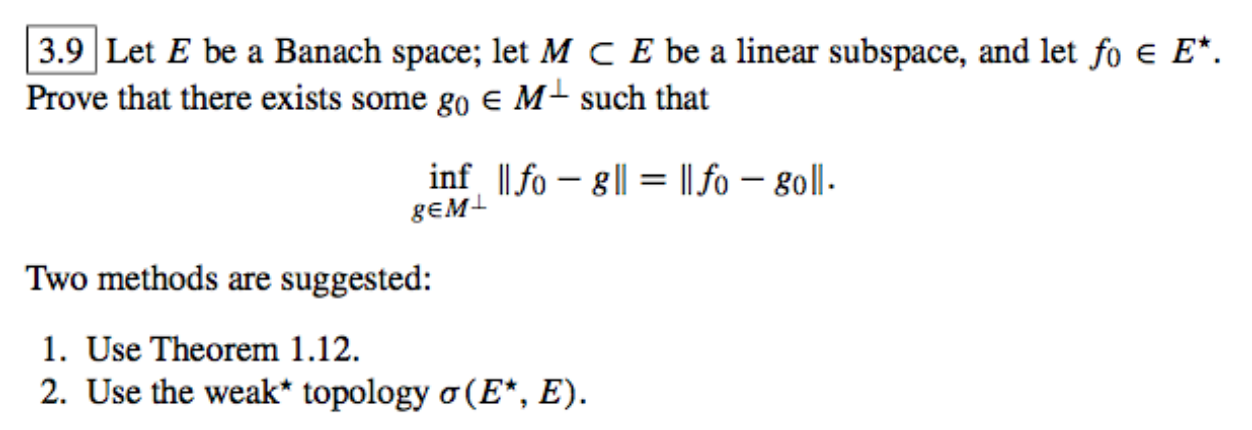
\includegraphics[width=0.7\textwidth]{funcA-h-e3-p2.png}
\end{figure}
\end{question}
\begin{solution} \hfill \\
Observe that
\eQb
M^{\perp} &=& \{ g \in E^* : <g,x> = 0 \> \forall x \in M\} \\ 
&=& \bigcap_{x \in M} \{g \in E^* : <g,x> = 0 \}  
= \bigcap_{x \in M} J(x)^{-1}(0) 
\eQe
where $J$ is the natural embedding. Hence, $M^{\perp}$ is weak-* closed. 
Choose $r_0 > 0$ such that 
\eQb
A &:=& B(f_0,r_0) \cap M^{\perp} \neq \emptyset.
\eQe
where $B(f_0, r_0)$ denotes closed ball of radius $r_0$ around $f_0$. Since 
closed balls are weak-* closed, $A$ is bounded and weak-* closed. Therefore,
by Banach-Alaoglu, $A$ is weak-* compact. 
Now, consider the map $\Phi:A \to \mathbb{R}$ defined by
\eQb
g &\mapsto& ||f_0 - g|| \>\>\>\> (g \in A).
\eQe
Observe that
\eQb
\{g \in A \> : \> \Phi(g) \leq \lambda \} &=& 
\{g \in A \> : \> ||f_0 - g|| \leq \lambda\} = 
B(f_0,\lambda) \cap A 
\eQe 
which is weak-* closed for all $\lambda \in \mathbb{R}$.
Hence, $\Phi$ is weak-* lsc, 
so there exists $g_0 \in A \subset M^{\perp}$ such that
\eQb
||f_0 - g_0|| &=& \inf_{g \in A} ||f_0 - g|| = \inf_{g \in M^{\perp}} ||f_0 - g||
\eQe
where the last equality holds by the choice of $A$.

\smallskip

In general, one should remark that Banach-Alaoglu implies that the dual norm
is lsc with respect to the weak-* topology. \hfill $\qed$

\end{solution}

\newpage

\begin{question}[3]
\hfill
\begin{figure}[h!]
  \centering
    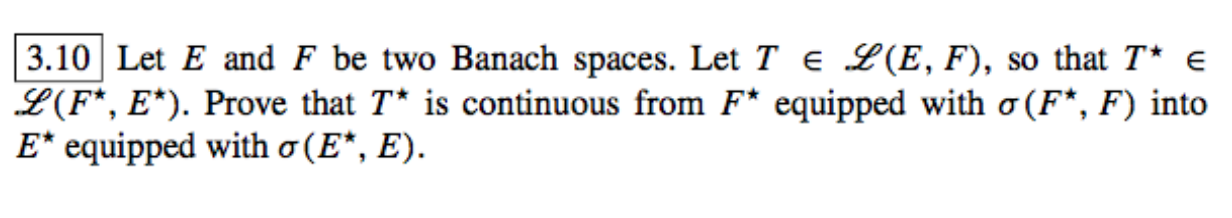
\includegraphics[width=0.7\textwidth]{funcA-h-e3-p3.png}
\end{figure}
\end{question}
\begin{solution} \hfill \\


\end{solution}

\newpage

\begin{question}[4]
\hfill
\begin{figure}[h!]
  \centering
    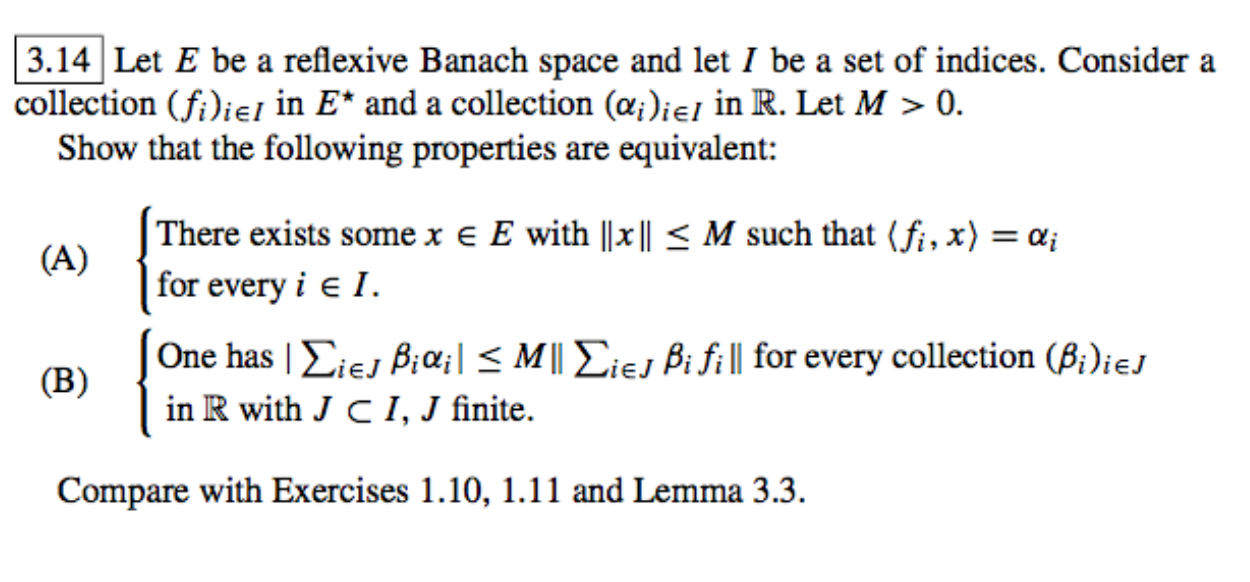
\includegraphics[width=0.7\textwidth]{funcA-h-e3-p4.png}
\end{figure}
\end{question}
\begin{solution} \hfill \\
$(A) \implies (B)$ is obvious. Fix $J$ finite, and $\{beta_i\}_{i \in J}$.
Then, use definition of norm and $(A)$, we get $(B)$.
For a moment, we assume the result of exercise 1.10
in Brezis.
Suppose (B) is true. Then, by 1.10, there exists $\phi_0 \in E^{**}$ such that 
\eQb
||f|| \leq M \>\>\> &\text{and}& \>\>\> <\phi_0,f_i> = \alpha_i
\eQe
for all $i \in I$. Then, by reflexivity of $E$, there exists $x_0 \in E$ such that
\eQb
||x_0|| \leq M  \>\>\> &\text{and}& \>\>\> <f,x_0> = \alpha_i 
\eQe
for all $i \in I$. Hence, it suffices to prove the result of 1.10. In particular,
we need $(B) \implies (A)$ direction. Let $G$ be the vector space spanned by
$\{x_i\}_{i \in I}$. Define $g:G \to \mathbb{R}$ by
\eQb
g(x) &=& \sum_{i \in J} \beta_i \alpha_i 
\eQe
where $x = \sum_{i \in J} \beta_i x_i$. $g$ is well-defined and bounded by assumption
(B). Now, extend $g$ to the whole of $E$ by corollary 1.2 of Hahn Banach, and 
we are done. \hfill $\qed$ 

\end{solution}

\newpage

\begin{question}[5]
\hfill
\begin{figure}[h!]
  \centering
    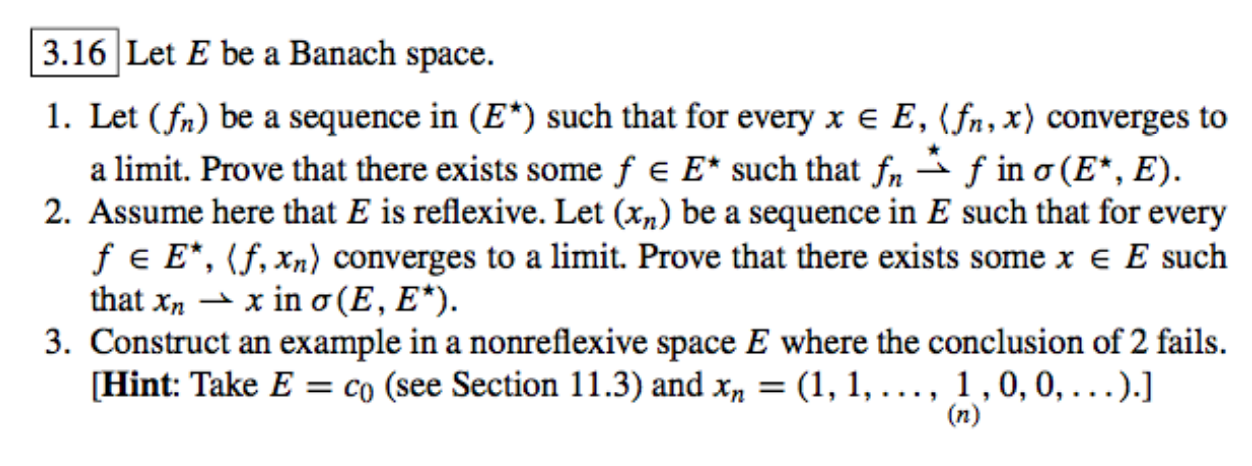
\includegraphics[width=0.7\textwidth]{funcA-h-e3-p5.png}
\end{figure}
\end{question}
\begin{solution} \hfill \\
\textbf{(i)}
Let $f:E \to \mathbb{R}$ be defined by
\eQb
<f,x> &=& \lim_{n \to \infty} <f_n,x> \>\>\> (x \in E).
\eQe
Then, $f$ is linear, because by linearty of $\{f_n\}$,
\eQb
<f,x+y> &=& \lim_{n \to \infty} <f_n,x+y> = \lim_{n \to \infty} <f_n,x> + <f_n,y> \\
&=& \lim_{n \to \infty} <f_n,x> + \lim_{n \to \infty} <f_n,y> = <f,x> + <f,y>
\eQe
for any $x,y \in E$ and
\eQb
<f,\lambda x> &=& \lim_{n \to \infty} <f_n,\lambda x> = \lambda \lim_{n \to \infty}
<f_N,x> = \lambda <f,x> 
\eQe
for any $\lambda \in \mathbb{R}$ and $x \in E$. Now, we prove the boundedness of $f$.
By the pointwise convergence,
\eQb
\sup_{n} |<f_n,x>| < \infty
\eQe
for all $x \in E$. 
Therefore, by uniform boundedness principle, there exists $C > 0$
such that
\eQb
|<f_n,x>| &\leq& C||x||
\eQe
and hence
\eQb
|<f,x>| &\leq& |<f_n,x>| + |<f_n,x> - <f,x>| \\
&\leq& C||x|| + |<f_n,x> - <f,x>| 
\eQe 
for any $x \in E$ and $n \geq 1$. Now, letting $n \to \infty$ gives 
\eQb
|<f,x>| &\leq& C||x||
\eQe
for any $x \in E$. 
Therefore, $f \in E^*$ such that 
\eQb
<f_n, x> \to <f,x> \>\>\> \text{as} \>\>\> n \to \infty 
\eQe
for any $x \in E$, which implies
\eQb
f_n \to_{\text{weak}-*} f \>\>\> \text{as} \>\>\> n \to \infty.
\eQe

\bigskip

\textbf{(ii)}
Set $\Phi:E^* \to \mathbb{R}$ by
\eQb
\Phi(f) &=& \lim_{n \to \infty} <f,x_n>.
\eQe
With uniform boundedness, and explicitly computing the limits 
as from above, $\Phi \in E^{**}$. Since the space is
reflexive, there exists $x \in E$ such that $J(x) = \Phi$. Then, by choice,
\eQb
<f,x_n> \to <f,x> \>\>\> \text{as} \>\>\> n \to \infty.
\eQe
therefore, $x_n \to_{\text{weak}} x$ as $n \to \infty$.

\bigskip

\textbf{(iii)} Let $E = C_0 \subset l^{\infty}$. Then, ${C_0}^{*} = l^1$, and
${C_0}^{**} = l^{\infty} \neq C_0$. Consider $\{x_n\}$ as in the hint. Let $u 
\in l^1$. Then,
\eQb
<u,x_n> &=& \sum_{k=1}^{n} u_k  
\eQe 
for all $n \geq 1$, and hence
\eQb
\lim_{n \to \infty} <u,x_n> &=& \sum_{k=1}^{\infty} u_k 
\eQe
which converges as $u \in l^1$. Hence, the hypothesis of (ii) is satisfied,
except for the fact that $E$ is not reflexive. Note that the i-th projections
$\{p_i\}$ are all trivially continuous. For $x_n$ to converge weakly to $x$,
it is necessary that
\eQb
\lim_{n \to \infty} <p_i,x_n> = x^{i} 
\eQe 
and hence
\eQb
x^{i} = 1
\eQe
for all $i \geq 1$.
As $x = (1,1,1,...) \not\in C_0$, there cannot exist $x \in E$ such that 
$x_n \to_{\text{weakly}} \to x$. \hfill $\qed$ 


\end{solution}

\newpage

\begin{question}[6]
\hfill
\begin{figure}[h!]
  \centering
    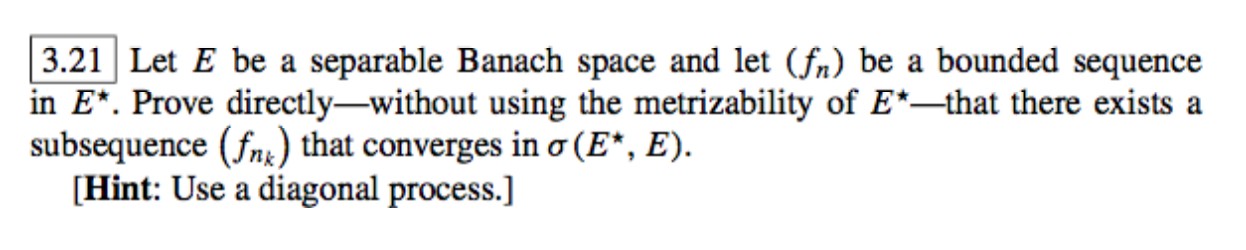
\includegraphics[width=0.7\textwidth]{funcA-h-e3-p6.png}
\end{figure}
\end{question}
\begin{solution} \hfill \\
By 3.16-1, it suffices to obtain a subsequence of $\{f_n\}$
such that $\{f_n\}$ converge pointwise everywhere.
As $E$ is separable, there exists $\{a_i\}$, 
a dense countable subset of $E$. 
Since $\{f_n\}$ are bounded in $E^*$, $\{<f_{n}, a_1> \}$ is bounded in $\mathbb{R}$.
Hence, we can choose a subsequence $\{n_k\}$, with relabeling $\{(1,k)\}$ such that 
\eQb
\lim_{k \to \infty} <f_{1,k},a_1> \>\>\> \text{exists}.
\eQe
Now, with the fact that $\{<f_{n},a_2 > \}$ is bounded in $\mathbb{R}$,
choose a further subsequence $\{n_{k_l}\}$ from $\{n_k\}$, with relabeling
$\{(2,k)\}$ such that
\eQb
\lim_{k \to \infty} <f_{2,k},a_2> \>\>\> \text{exists}.
\eQe
Repeat this process inductively, so that we have chosen $f_{l,k}$ for all $l,k \in
\mathbb{N}$. Then, consider $\{ g_{l} \} = \{f_{l,l}\}$, 
which is the standard diagonal sequence. 
Then, by choice
\eQb
\lim_{l \to \infty} <g_l, a_i> \>\>\> \text{exists}
\eQe 
for any $i \in \mathbb{N}$. Now, let $a \in E$, and $\epsilon > 0$.
Choose $a_i$ such that $||a_i - a|| < \epsilon$. Then,
\eQnb
|<g_n,a> - <g_m,a>| &\leq& |<g_n, a> - <g_n,a_i>| + |<g_m, a_i> - <g_m, a>|
\nonumber \\
&+& |<g_n, a_i> - <g_m,a_i>| \nonumber \\
&\leq& |<g_n, a - a_i>| + |<g_m, a_i - a>|  \label{eq:6.1} \\ 
&+& |<g_n, a_i> - <g_m,a_i>| \nonumber \\
&\leq& 2C\epsilon + |<g_n, a_i> - <g_m,a_i>| \label{eq:6.2} 
\eQne
for all $n,m \geq 1$, where~\eqref{eq:6.1} holds by linearity, 
and~\eqref{eq:6.2} holds by the choice of $a_i$
and $C$ being the bound on the $\{f_n\}$ in the dual norm. Therefore, 
\eQb
|<g_n,a> - <g_m,a>| &\leq& (2C + 1)\epsilon
\eQe 
for all $n,m$ large enough, and hence, we have shown that 
\eQb
<g_l, a> \>\>\> \text{converges to a limit} \>\>\> \text{as} \>\>\> l \to \infty 
\eQe 
for any $a \in E$. Hence, we are done. \hfill $\qed$
 

\end{solution}



\end{document}
